
\documentclass[10pt]{article}
\usepackage[margin=1in]{geometry}
\usepackage{amsmath}
\usepackage{amssymb}
\usepackage{setspace}
\usepackage{graphicx}
\usepackage{caption}
\usepackage{listings}


\begin{document}

\title{ECE 4750 Lab 3: Blocking Cache}
\author{Avinash Navada (abn44) \& Akshay Dongaonkar (akd54) \& Vivek Gaddam (vrg22)}
\maketitle


\section{Introduction}

One of the main factors affecting processor performance is memory latency. Accessing main memory can take hundreds of cycles, which could potentially reduce the impact of any ingenious processor architectural modifications. One way to reduce the effect of this memory delay is to incorporate a cache into the architecture: a relatively small, fast memory (usually SRAM) that holds instructions and/or data that the processor can access without having to go to the (slower) main memory. Since caches are much smaller than main memory, the cache controller needs to be selective about the type of data that is stored and so aims to capitalize on temporal and spatial locality when fetching cache lines. In this lab, we design and synthesize two different cache architectures.  \\

Our baseline design was a direct-mapped cache and our alternative design was a two-way set-associative cache, both of 256B capacity. In a direct-mapped cache, any location in memory maps to exactly one location in the cache, whereas in a n-way set-associative cache, any location in memory can map to one of n different locations (or ways). This means that there would be less conflict misses with the set-associative cache since multiple memory locations with the same index bits can be mapped to the cache simultaneously, which would lead to an improvement in the average memory access latency (AMAL) over a direct-mapped cache. Therefore we expect an improvement in the AMAL for our two-way set-associative cache design over the direct-mapped cache design.


\section{Project Management}

We assigned Vivek to be the architect, Akshay to be the verification lead, and Avinash to be the design lead.
Our initial project roadmap was rather aggressive and required us to be finished by Sunday, October 26\textsuperscript{st}, since we planned on trying out an extension or two for this lab. The Gantt Chart with both the planned and actual roadmaps overlaid is shown in Figure~\ref{fig:gantt}. Clearly, we couldn't meet the aggressive deadlines we set initially although we did manage to complete the lab before the actual deadline. \\

The work was divided as follows:
Vivek worked on the random testing and part of the writeup.
Akshay worked on most of the baseline implementation and alternative implementations, and created the directed testing suite for the baseline implementation.
Avinash wrote most of the writeup, worked on part of the baseline implementation, and created the directed testing suite for the alternative implementation.
All team members worked on debugging the RTL logic and test cases. \\

The work was approached by simultaneously starting the baseline implementation and testing, followed by the lab writeup shortly after. Baseline paths that were completed were promptly tested. As soon as the baseline implementation was complete and successfully tested, we moved on to the alternative design implementation and testing (which included adding additional test cases for the alternative design). Even though we assigned different roles to each of the team members, different team members took the initiative to work on different aspects of the lab and so we all ended up getting a thorough understanding of all parts of the lab. Starting the lab earlier would have allowed us to build some extensions, although we are glad we were able to finish the assigned work on time and were able to test and evaluate our designs thoroughly. 


\section{Baseline Design}

The baseline design for this lab is a 256B direct-mapped, write-back, write-allocate cache. The baseline design was split into control, datapath, and top-level modules to make design and debugging easier but also to enforce the design principles of modularity, hierarchy, and encapsulation for a design of this level of complexity. The cache control is managed by a finite state machine (FSM) controller that deals with states with one or more steps per state during which control signals are fed out to the datapath and status signals are received in return. State machine and datapath diagrams for the baseline design are shown in Figures \ref{fig:state} and \ref{fig:baseline} and respectively. We utilize val/ready interfaces for instruction/data memory requests which allows memory systems of varying latencies to be composed with the cache.The interface for the direct-mapped cache consists of the following inputs: clock and reset signals, the test source/cache request message and valid signal, cache response ready signal (from the test sink/processor), memory request ready signal, and the memory response message and valid signal. The outputs are: the cache request ready signal, cache response message and valid signal, memory request message and valid signal, as well as the memory response ready signal. We began working on the design by first fully creating the datapath and then adding the different paths: init transaction, read hit path, write hit path, refill path, and evict path. Since the cache is write-back, write-allocate, we write only to the cache on a write hit and load the cache line from memory (and then write to the cache) on a write miss. Also, we maintain two register files in the control module for keeping track of valid and dirty cache lines. This information is necessary for determining whether evictions are required on cache read/write misses. \\


\section{Alternative Design}

The alternative design for this lab is a 256B two-way write-back, write-allocate set-associative cache. Just like the baseline design, the alternative design was split into control, datapath, and top-level modules, with control being managed by a FSM controller. The alternative design has a least recently used (LRU) replacement policy for choosing which cache lines to replace on read/write misses. State machine and datapath diagrams for the alternative design are shown in Figures \ref{fig:state} and \ref{fig:alt} respectively. The state diagram is the same for both the baseline and alternative designs since the only difference in their control logic lies in that hit and miss transitions are defined differently: for the baseline design, there is only one tag array to get a hit/miss from whereas for the alternative design, we would get a hit if either tag array has registered a hit and a miss if both tag arrays register misses. 
The main datapath changes that had to be made to the baseline design to create the alternative design involved duplicating the tag array and tag check logic. The modifications made to the control logic were more extensive, however. These modifications include having different valid, dirty, and count (for LRU) register files for each way, more complex logic to determine which way to write to, and logic to implement the LRU replacement policy. Furthermore, we tried to improve the modularity of our design by refactoring the tag/data arrays and output logic into separate ``way modules'' (in file ``lab3-mem-BlockingCacheAltWay.v''), which reduced the chance of errors and confusion during design. These way modules can be seen in the alternative design datapath diagram shown in Figure \ref{fig:alt}, while a sneak-peek into a way module itself is shown in Figure \ref{fig:way}.  \\


\section{Testing Strategy}

We began the testing process by writing and running directed tests for each of the 5 different paths (init, hit, miss, refill, evict) as they were implemented. These tests were first run on the functional model to ensure correctness after which they were run on the baseline implementation. A similar process was carried out for the alternative implementation. The first 6 directed test cases we wrote tested read/write hit/miss functionality for clean/dirty cases. These test cases were aimed at the baseline implementation while the rest of our test cases were aimed at the alternative implementation; even though all the tests are needed to ultimately forge comparisons between the baseline and alternative designs, the test cases aimed at the alternative design were intended to test certain characteristics specific to a set-associative cache, e.g. testing control logic for determining the source of conflict misses (in either way) and testing the least recently used (LRU) replacement policy. We ensured that read misses were correctly handled by the cache controller with a LRU replacement policy by filling up both cache ways for one set of instructions and causing read misses to those cache lines. However, in order to specifically target the LRU control logic, i.e. determine whether or not the least recently used cache line is selected correctly, we modified the alternative design control logic to output \texttt{h'0a} if the way 0 cache line was replaced and a \texttt{h'0b} as opaque bits if the way 1 cache line was replaced. We then created directed tests that wrote the expected opaque bits to the test sink to verify correct implementation of the LRU replacement policy. This modification was clearly meant for test purposes only and so we removed the code for these special tests once we were done testing. We also made two additional states called FAIL0 and FAIL1 in the baseline implementation so that we could use trace instead of gtkwave to debug (and observe the states). \\

Following completion of the directed tests, we were able to write and run random tests. Specifically, these tests randomized memory accesses, the type of accesses, and data values written/read in memory. This was done by modifying the provided Python script \texttt{lab3-mem-gen-input.py} to take additional arguments specifying a particular random test and putting the resulting Python code in a separate python file \texttt{ubmark-randtest-suite.py}. As a result, we were able to generate a couple varieties of random tests to more broadly evaluate our design. The first random test simply loaded random data across a fixed memory address space and then made sequential (word) accesses in that address space. The second random test goes a few steps further. Like the previous test, it started by loading random data across a fixed memory address space. However, it then randomized both the addresses of data accesses within that space and the type of access (read or write). While doing all this, it did not allow a particular address to be accessed more than twice for either type of access - this effectively ``spreads'' accesses across the address space, yet still allows for scenarios where a particular memory address that was initialized to a particular value would be overwritten and read.

																	% BUGS


Ultimately both the base and alternative designs worked correctly with all test cases.  \\


\section{Evaluation}

As soon as the baseline and alternative implementations were completed, we proceeded to test the performance of the models. In order to achieve this, the simulator harness was built and run (using the given datasets) to generate the total number of cycles and the average number of cycles per transaction for the base and alternative designs. We also added our own datasets to the harness to compare the performance of the two models in different targeted scenarios. The results of the simulator for each dataset and design are summarized in Table~\ref{tab:eval} and the Average Memory Access Latency (AMAL) results are summarized in Table \ref{tab:amal} for clarity. As Table~\ref{tab:eval} shows, we tested the baseline and alternative implementations on the loop-1D, loop-2D, and loop-3D datasets. These datasets access sequential memory locations based on an offset/s for n-dimensions (where n $\epsilon$ \{1,2,3\}). Therefore we expected to see much slower performance for both the baseline and alternative implementations as n is increased. \\

The results in Table~\ref{tab:eval} clearly show the performance improvement of the alternative implementation over the baseline implementation. The number of cycles utilized was more or less the same for both implementations for all but the loop-3d dataset. The number of cache accesses were the same for both models as expected (by design). Now the number of hits were far greater and the number of misses were far less for the alternative implementation over the baseline implementation. 

One possible explanation for the less-than-stellar performance difference of the set-associative cache over the direct-mapped cache is that this difference will be better seen for small datasets since the alternative implementation is of low associativity (2 ways).  

% Since we are comparing different pipelined processors on the \textit{same program}, the only factors affecting our performance are the cycle time (CT) and cycles per instruction (CPI).
% To a first approximation, we can assume that the clock cycle time is the same across the processors. \\

% If we make that approximation, the only factor left is cycles per instruction. 
% If we look at Table~\ref{tab:cycles}, our fully bypassed processor has the higest CPI.
% However, it is interesting to look at the performace as various bypass paths are implemented.
% Looking at vvadd-unopt, we see that after the first bypass path is implemented, its performance stagnates.
% This i s because CPI is incredibly reliant on the program that is running. 
% We need to remember this when we run our benchmarks. 
% They may not be representative of programs in the wild. 
% However, assuming that our benchmarks do mirror programs running on our processor, the fully bypassed processor performs equally or better than other processors in all cases. Better is defined as having a lower CPI. \\

% Our first approximation may not be correct though!
% We may have added a critical path to our datapath when we added a bypass.
% Looking at our datapath diagram, we postulate that our critical path goes through the multiplier.
% This is reinforced by the results of the complex multiply benchmark.
% We waste about three cycles obtaining a result from the multiplier.
% However, since we use a val/rdy microprotocol, if the multiplier is not being used we can reduce our clock cycle time.
% We postulate then that our critical path for non val/rdy microprotocol affected components includes the ALU, the bypass into op1, and the mux selecting between the two.
% This may affect performance. We need to do a better study of the tradeoffs to correctly predict.


\pagebreak[4]


\section {Tables and Diagrams}


% % Table: Eval - Performance

\begin{table}[h]
\begin{center}
\begin{tabular} {|l | r | r | r | r | r | r | r | r | r | r |}

\hline
\textbf{Design}    & \textbf{Cycles} & \textbf{Cache} & \textbf{Hits} & \textbf{Misses} & \textbf{Miss} & \textbf{Memory} & \textbf{Refills} & \textbf{Evicts} & \textbf{AMAL} \\
&&\textbf{Accesses}&&&\textbf{Rate}&\textbf{Accesses}&&& \\
\hline
Baseline - loop 1D       &  951   &  100   &  75   &  25  &	 25.0\%  &  25  &  25  &  0  &  9.510000	\\
Baseline - loop 2D 	     &  4135  &  500   &  403  &  97  &	 19.4\%  &  97  &  97  &  0  &  8.270000	\\
Baseline - loop 3D       &  2081  &  80    &  0    &  80  &	 100.0\% &  80  &  80  &  0  &  26.012500	\\
\hline
Alternative - loop 1D    &  951   &  100   &  75   &  25  &	 25.0\%  &  25  &  25  &  0  &  9.510000	\\
Alternative - loop 2D    &  4751  &  500   &  375  &  125 &	 25.0\%  &  125 &  125 &  0  &  9.502000	\\
Alternative - loop 3D    &  673   &  80    &  64   &  16  &	 20.0\%  &  16  &  16  &  0  &  8.4125000	\\
\hline                    
\end{tabular}
\caption{Baseline v. Alternative Design Performance}
\label{tab:eval}
\end{center}
\end{table}


% % Table: Eval - Performance/AMAL

\begin{table}[h]
\begin{center}
\begin{tabular} {|l | r |}

\hline
\textbf{Design} & \textbf{AMAL} \\
\hline
lab3-mem-sim-base-loop-1d.out & 9.510000  \\
lab3-mem-sim-base-loop-2d.out & 8.270000  \\
lab3-mem-sim-base-loop-3d.out & 26.012500 \\
lab3-mem-sim-alt-loop-1d.out  & 9.510000  \\
lab3-mem-sim-alt-loop-1d.out  & 9.502000  \\
lab3-mem-sim-alt-loop-1d.out  & 8.412500  \\
\hline
\end{tabular}
\caption{Baseline v. Alternative Design AMAL}
\label{tab:amal}
\end{center}
\end{table}



% % Figure: Gantt Chart

\begin{figure}[b]
\centering
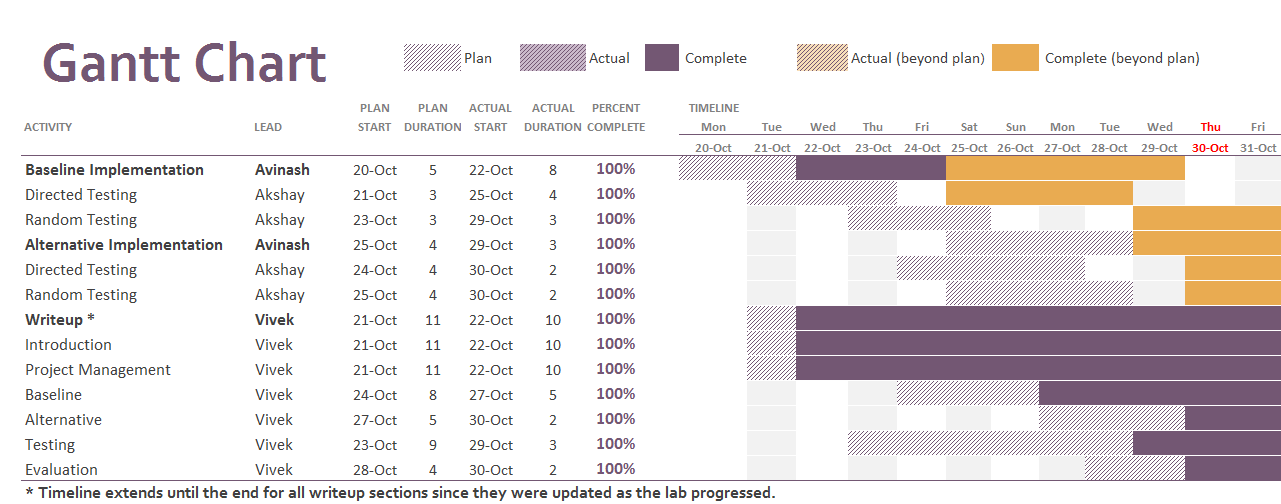
\includegraphics[scale=0.5, angle=90]{gantt}
\caption{Gantt Chart}
\label{fig:gantt}
\end{figure}

% Figure: FSM Control Unit State Diagram

\begin{figure}[b]
\centering
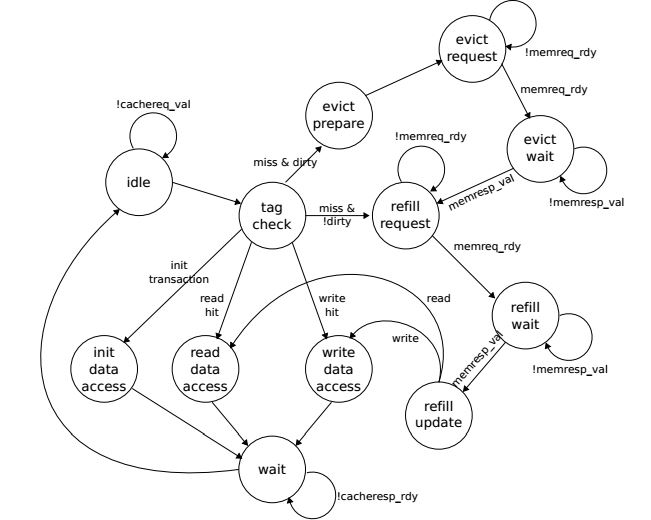
\includegraphics[scale=0.8]{state}
\caption{Baseline FSM Control Unit State}
\label{fig:state}
\end{figure}

% % Figure: Baseline Design Datapath Diagram

\begin{figure}[b]
\centering
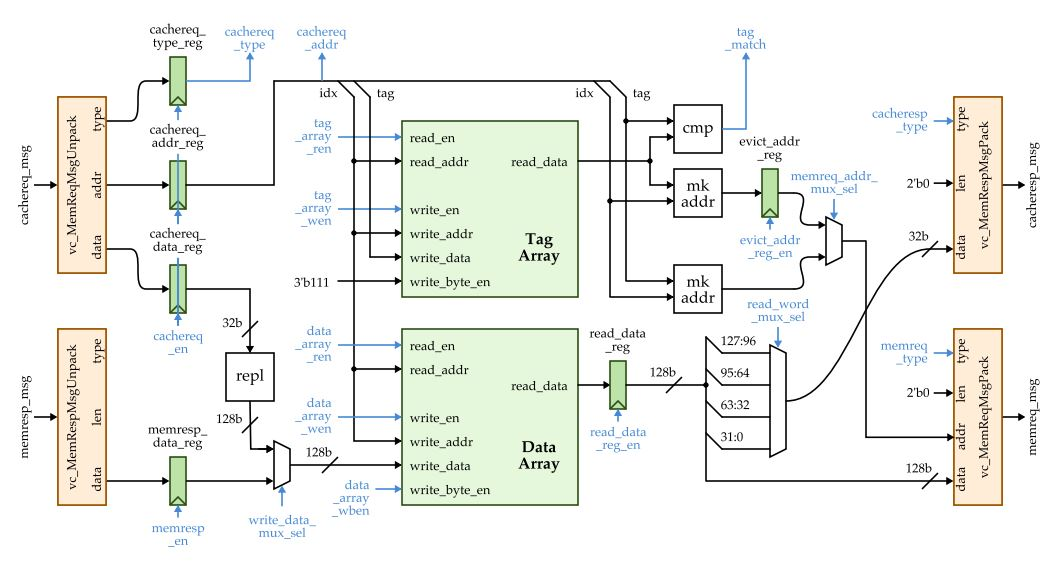
\includegraphics[scale=0.6]{baseline}
\caption{Baseline Design Datapath}
\label{fig:baseline}
\end{figure}


% % Figure: Alternative Design Datapath Diagram

\begin{figure}[b]
\centering
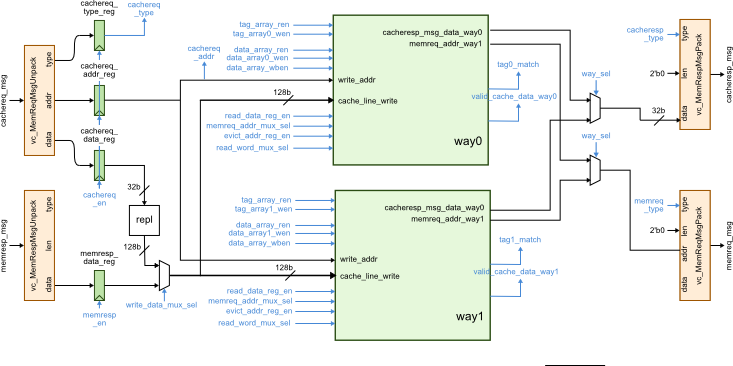
\includegraphics[scale=0.8]{alt}
\caption{Alternative Design Datapath}
\label{fig:alt}
\end{figure}

% % Figure: Way Module

\begin{figure}[b]
\centering
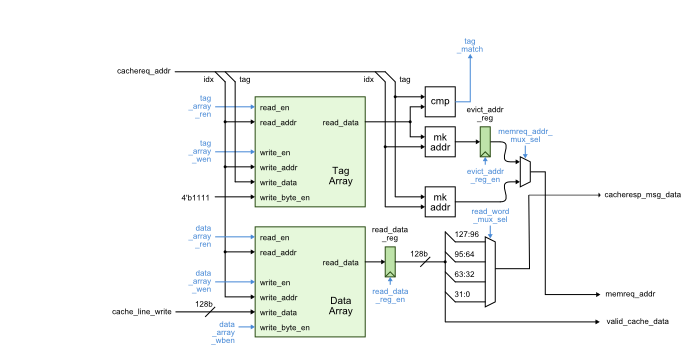
\includegraphics[scale=0.9]{way}
\caption{Way Module}
\label{fig:way}
\end{figure}


\end{document}






